\documentclass[12pt]{article}
\usepackage{graphicx}
\usepackage{caption}
\usepackage{subcaption}
\usepackage{tikz}
\usepackage{tcolorbox}
\usepackage{listings}
\usepackage{amsmath}
\usepackage{amssymb}
\usepackage{xcolor}
\usepackage[margin=1cm, top=1.5cm, bottom=1.5cm]{geometry}

\tcbuselibrary{breakable}

\title{\textbf{Gráficas y Juegos: Participación 02}}
\author{Rendón Ávila Jesús Mateo}
\date{\today}

\begin{document}

\maketitle
\begin{center}
\vspace{3cm}
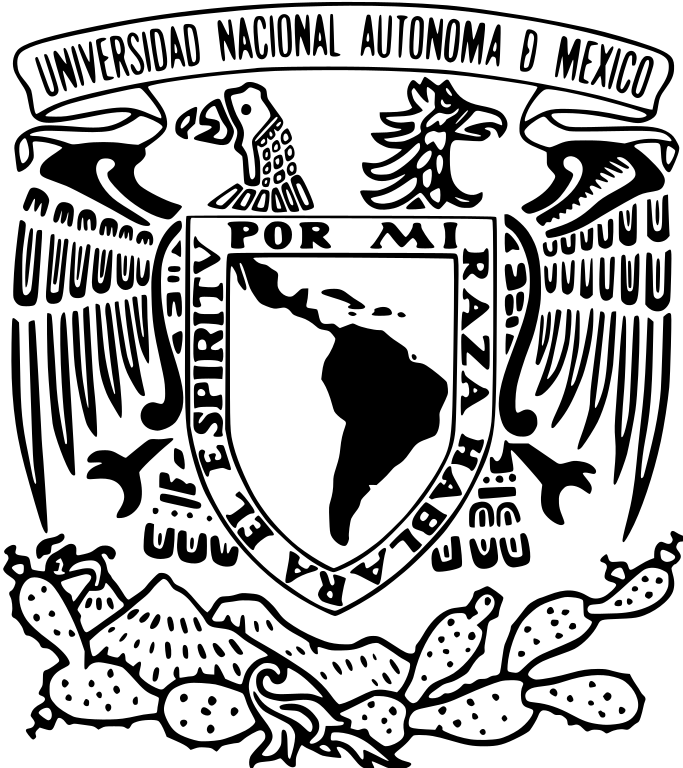
\includegraphics[width=0.195\textwidth]{Escudo.png}
\hspace{0.5cm}
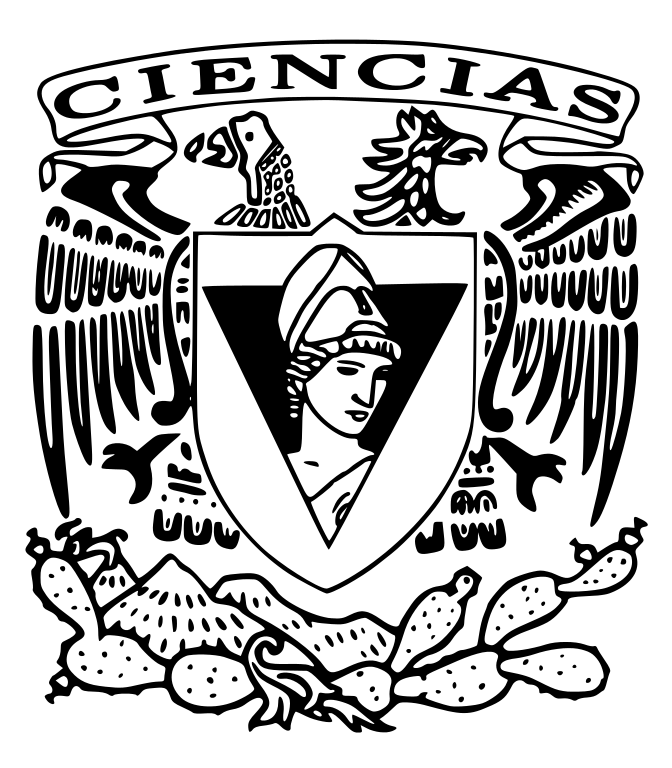
\includegraphics[width=0.2\textwidth]{logo_ciencias.png}
\end{center}
\begin{center}
    \vspace{1cm}
    Universidad Nacional Autónoma de México\\
    Facultad de Ciencias\\
    Profesor: César Hernández Cruz\\
\end{center}

\newpage

%
% Ejercicio 1
%
\textbf{1.} Sea $D$ una digráfica cualquiera, demuestra que si $D$ no tiene vértices con ingrado cero, entonces $D$ contiene un ciclo dirigido.

\begin{tcolorbox}[title=\textbf{Hipotesis}, colback=red!15!white, colframe=black!]
    1. $D$ es una digráfica, $i.e$ $D$ es una pareja ordenada $D = (V(D), A(D))$ donde $V(D)$ es un conjunto arbitrario y $A(D)$ es un subconjunto de $V(D) \times V(D) - L$ 
    donde $L = \{(v,v) \mid v \in V(D)\}$.\\

    2. Para todo elemento $v \in V(D)$, sabemos que $d^-(v) \neq 0$
\end{tcolorbox}

Sabemos que $D$ tiene que tener una dirección para cada arista $(v, v') \in A(D)$, por lo que si existriera una secuencia de vértices
$\{v_1, v_2, \ldots, v_n\}$ sabemos que $(v_1, v_2), (v_2, v_3), \ldots, (v_{n-1}, v_n) \in A(D)$, pero si fuera así entonces 
$d^-(v_1 = 0)$ lo cual es una contradicción con la hipótesis. Así que debe ser $(v_n, v_1) \in A(D)$.\\

Por lo tanto podemos afirmar que $D$ tiene un ciclo dirigido para alguna secuencia de vértices $\{v_1, v_2, \ldots, v_n\}$ para toda $v_i$ tal que $i \in \{1, 2, 3, \ldots, n\}$
con $n \leq \mid V(D) \mid$.

\end{document}